\scanpage{128}
\mspage{127}

\uline{Graphes} MD

Un \uline{graphe} \uline{pondéré} est donné par
\[
(1)\qquad (S,\widehat{\vec A},o,\sigma,g)
\]
i.e. $S,\widehat{\vec A}$ ens. finis, $o:\widehat{\vec A}-S$ application (``origine''),
$\sigma:\widehat{\vec A}-\widehat{\vec A}$ une involution, $g:S\longrightarrow\mathbb N$ une application :

(2)\quad
\diagram{\begin{tikzcd}[column sep=large,row sep=large]
\overset{\text{arcs}}{\widehat{\vec A}}
 \arrow[r,"o","\substack{\text{appl.}\\\text{origine}}"']
 \arrow[loop below,"\sigma","\substack{\text{passage}\\\text{à l'arc opposé}}"']
& \overset{\text{sommets}}{S}
 \arrow[r,"\uline{g}","\substack{\text{application}\\\text{``genre''}}"']
& \mathbb N
\end{tikzcd}}
\[
.\quad \sigma^2=\mathrm{id}_{\vec A}
\]

\margin{On pose
$\left\{\begin{array}{l}
\widehat{\vec A}^{\sigma}=I\hookrightarrow\widehat A\\
\vec A=\unsure{\widehat{\vec A}}\setminus\unsure{\widehat{\vec A}}^{\sigma}\\
A=\vec A/\sigma\simeq\widehat A\setminus I
\end{array}\right.$}

On pose
\[
(3)\qquad \widehat{\vec A}/\sigma=\widehat A\qquad(\text{arêtes})
\]
arêtes \uline{ordinaires} \inserted{ou \uline{liées}} sont les arêtes correspondant à des orbites à deux éléments, les autres sont dites \deleted{\uline{\unsure{bouts|boucles}}} \deleted{\uline{\unsure{plats}}} arêtes libres. Représentation graphique
\margin{\uline{NB} On ne marque pas $g_i$ si $g_i=0$.}
\figure{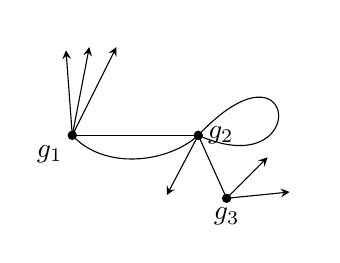
\begin{tikzpicture}[x=0.8cm,y=0.8cm,>=stealth]
\coordinate (s1) at (0,0);\coordinate (s2) at (2,0);\coordinate (s3) at (2.45,-1);
\draw (s1)--(s2);\draw (s1) .. controls (0.5,-0.55) and (1.5,-0.45) .. (s2);
\draw (s2) .. controls (3.6,1.7) and (3.8,-0.8) .. (s2);
\draw (s2)--(s3);
\draw[->] (s1)--(-0.1,1.35);\draw[->] (s1)--(0.27,1.4);\draw[->] (s1)--(0.7,1.4);
\draw[->] (s2)--(1.5,-0.95);\draw[->] (s3)--(3.1,-0.35);\draw[->] (s3)--(3.45,-0.9);
\fill (s1) circle (1.7pt);\fill (s2) circle (1.7pt);\fill (s3) circle (1.7pt);
\node[below left] at (s1) {$g_1$};\node[right] at (s2) {$g_2$};\node[below] at (s3) {$g_3$};
\end{tikzpicture}}

\margin{\deleted{\unsure{orientations}} \unsure{pondérés} \uline{\unsure{comme d'hab.}} \deleted{\unsure{MD}}}

Condition de stabilité MD :
\[
(4)\qquad \forall s\in S,\ \text{on a }2g_s+\widehat\nu_s\geq3\quad\text{i.e.}\quad
\left\{\begin{array}{l}
g_s=0\ \Rightarrow\ \widehat\nu_s\geq3\\
g_s=1\ \Rightarrow\ \widehat\nu_s\geq1
\end{array}\right.
\]
\margin{graphes \uline{stables} : qui satisfont la condition (4)}

i.e. $\widehat\nu_s$ est le nb d'arcs \deleted{qui} d'origine $s$ (\uline{ordre total} du sommet $s$) tandis que $\nu_s$ désignera le nb d'arcs ordinaires, donc
\[
(5)\qquad
\underset{\substack{\uline{\text{ordre total}}\\\text{de }s}}{\widehat\nu_s}
=
\underset{\substack{\uline{\text{ordre}}\\\deleted{\unsure{\text{total}}}\\\uline{\unsure{\text{réduit}}}\\\text{de }s}}{\nu_s}
+
\overset{\substack{\unsure{\operatorname{card}I}\ \text{si }I=\widehat{\vec A}^{\sigma}}}{
\underset{\substack{\uline{\text{ordre complémentaire}}\\\text{de }s\\\text{(correspondant}\\\text{aux ``pts marqués''}\\\text{sur une courbe alg.)}}}{\unsure{\vec\nu_s}}}
,\quad \uline{\text{``marqué''}}
\]
\deleted{$\unsure{\nu_s}=2\unsure{\nu'_s}\quad\unsure{\nu'_s}\ \unsure{\text{nb d'arêtes}}$}

\margin{Si le graphe est connexe, le couple $(g,\nu)$ est \unsure{appelé} son type numérique. Dans le cas général, on lui associe \unsure{l'invariant numérique}, \unsure{spécifié} par une application
\diagram{\begin{tikzcd}
\uline{I}\arrow[r]&\pi_0(G)\arrow[r,"g","\substack{\text{genre}\\\text{virtuel}\\\text{d'une}\\\text{composante}}"']&\mathbb N
\end{tikzcd}}}

On pose
\[
(6)\qquad \nu=\nu(G)\deleted{\unsure{\nu_G}}=\sum_s\unsure{\vec\nu_s}=\operatorname{card}(\vec A^{\sigma})\quad
(\uline{\text{ordre marqué}}\ \deleted{\unsure{\text{tot}}}\ \text{du graphe})
\]
\[
(7)\qquad c=c(G)=\deleted{\unsure{\nu}}\frac12\sum_s\nu_s
\qquad\text{nb des arêtes ordinaires : }\uline{\text{codim.}}\ \uline{\text{modulaire}}\ \text{du graphe}
\]
\[
(8)\qquad g=\sum_{s\in S}g_s+\underset{\substack{\unsure{\text{connexité}}\\\text{de }G}}{\underbrace{h^1(G)}}.
\quad\uline{\text{genre virtuel}}\ \text{du graphe}
\]
(correspond à $\dim H^1(X,\unsure{\mathcal O_X})$)
